\documentclass{article}\usepackage[]{graphicx}\usepackage[]{xcolor}
% maxwidth is the original width if it is less than linewidth
% otherwise use linewidth (to make sure the graphics do not exceed the margin)
\makeatletter
\def\maxwidth{ %
  \ifdim\Gin@nat@width>\linewidth
    \linewidth
  \else
    \Gin@nat@width
  \fi
}
\makeatother

\definecolor{fgcolor}{rgb}{0.345, 0.345, 0.345}
\newcommand{\hlnum}[1]{\textcolor[rgb]{0.686,0.059,0.569}{#1}}%
\newcommand{\hlsng}[1]{\textcolor[rgb]{0.192,0.494,0.8}{#1}}%
\newcommand{\hlcom}[1]{\textcolor[rgb]{0.678,0.584,0.686}{\textit{#1}}}%
\newcommand{\hlopt}[1]{\textcolor[rgb]{0,0,0}{#1}}%
\newcommand{\hldef}[1]{\textcolor[rgb]{0.345,0.345,0.345}{#1}}%
\newcommand{\hlkwa}[1]{\textcolor[rgb]{0.161,0.373,0.58}{\textbf{#1}}}%
\newcommand{\hlkwb}[1]{\textcolor[rgb]{0.69,0.353,0.396}{#1}}%
\newcommand{\hlkwc}[1]{\textcolor[rgb]{0.333,0.667,0.333}{#1}}%
\newcommand{\hlkwd}[1]{\textcolor[rgb]{0.737,0.353,0.396}{\textbf{#1}}}%
\let\hlipl\hlkwb

\usepackage{framed}
\makeatletter
\newenvironment{kframe}{%
 \def\at@end@of@kframe{}%
 \ifinner\ifhmode%
  \def\at@end@of@kframe{\end{minipage}}%
  \begin{minipage}{\columnwidth}%
 \fi\fi%
 \def\FrameCommand##1{\hskip\@totalleftmargin \hskip-\fboxsep
 \colorbox{shadecolor}{##1}\hskip-\fboxsep
     % There is no \\@totalrightmargin, so:
     \hskip-\linewidth \hskip-\@totalleftmargin \hskip\columnwidth}%
 \MakeFramed {\advance\hsize-\width
   \@totalleftmargin\z@ \linewidth\hsize
   \@setminipage}}%
 {\par\unskip\endMakeFramed%
 \at@end@of@kframe}
\makeatother

\definecolor{shadecolor}{rgb}{.97, .97, .97}
\definecolor{messagecolor}{rgb}{0, 0, 0}
\definecolor{warningcolor}{rgb}{1, 0, 1}
\definecolor{errorcolor}{rgb}{1, 0, 0}
\newenvironment{knitrout}{}{} % an empty environment to be redefined in TeX

\usepackage{alltt}
\usepackage{amsmath} %This allows me to use the align functionality.
                     %If you find yourself trying to replicate
                     %something you found online, ensure you're
                     %loading the necessary packages!
\usepackage{amsfonts}%Math font
\usepackage{graphicx}%For including graphics
\usepackage{hyperref}%For Hyperlinks
\usepackage[shortlabels]{enumitem}% For enumerated lists with labels specified
                                  % We had to run tlmgr_install("enumitem") in R
\hypersetup{colorlinks = true,citecolor=black} %set citations to have black (not green) color
\usepackage{natbib}        %For the bibliography
\setlength{\bibsep}{0pt plus 0.3ex}
\bibliographystyle{apalike}%For the bibliography
\usepackage[margin=0.50in]{geometry}
\usepackage{float}
\usepackage{multicol}

%fix for figures
\usepackage{caption}
\newenvironment{Figure}
  {\par\medskip\noindent\minipage{\linewidth}}
  {\endminipage\par\medskip}
\IfFileExists{upquote.sty}{\usepackage{upquote}}{}
\begin{document}

\vspace{-1in}
\title{Lab 7-8 -- MATH 240 -- Computational Statistics}

\author{
  Yuliia Heleveria \\
  MATH 240 Lab A  \\
  Mathematics  \\
  {\tt yheleveria@colgate.edu}
}

\date{04/01/2025}

\maketitle

\begin{multicols}{2}
 \raggedcolumns
\begin{abstract}
This document provides a basic template for the 2-page labs we will complete each week. Here, briefly summarize what you did and why it might be helpful. Provide all the top-line conclusions, but avoid providing \emph{all} the details. Results should be limited to ``we show X, Y, and Z."
\end{abstract}

\noindent \textbf{Keywords:} What topics does the lab cover concerning class? List 3-4 key terms here, separated by semicolons.

\section{Introduction}
The Beta distribution is a continuous distribution that is defined on the interval [0,1]. It is used to model a random variable \textit{X}. The Beta distribution is used to model proportions, rates, and probabilities. The distribution is governed by two shape parameters: $\alpha > 0$ and $\beta > 0$, which determine the shape for different data distributions. The Beta distribution is very flexible with its shape: it can be left-skewed, right-skewed, or symmetric. 


Section \ref{sec:pdf} defines the probability density function (PDF) and its parameters for Beta distribution. Section \ref{sec:prop} covers statistical characteristics of the Beta distribution such as mean, variance, skewness, and excess kurtosis. Section \ref{sec:estim} discusses the methods for estimating $\alpha$ and $\beta$ from sample data using the method of moments (MOM) and maximum likelihood estimation (MLE). Section \ref{sec:examp} presents the example from the death rates data to demonstrate parameter estimation.



\section{Density Function and Parameters}\label{sec:pdf}
The probability density function (PDF) of Beta distribution is given by the formula:

\[
 f(x | \alpha, \beta) = \frac{\Gamma(\alpha + \beta)}{\Gamma(\alpha)\Gamma(\beta)} x^{\alpha-1}(1-x)^{\beta-1} I(x \in [0,1]),
\]
where $I(x \in [0,1]) = 1$ when $x \in [0,1]$ and 0 otherwise.

The shape parameters $\alpha$ and $\beta$ control the skewness and concentration of the distribution.


\begin{Figure}
 \centering
 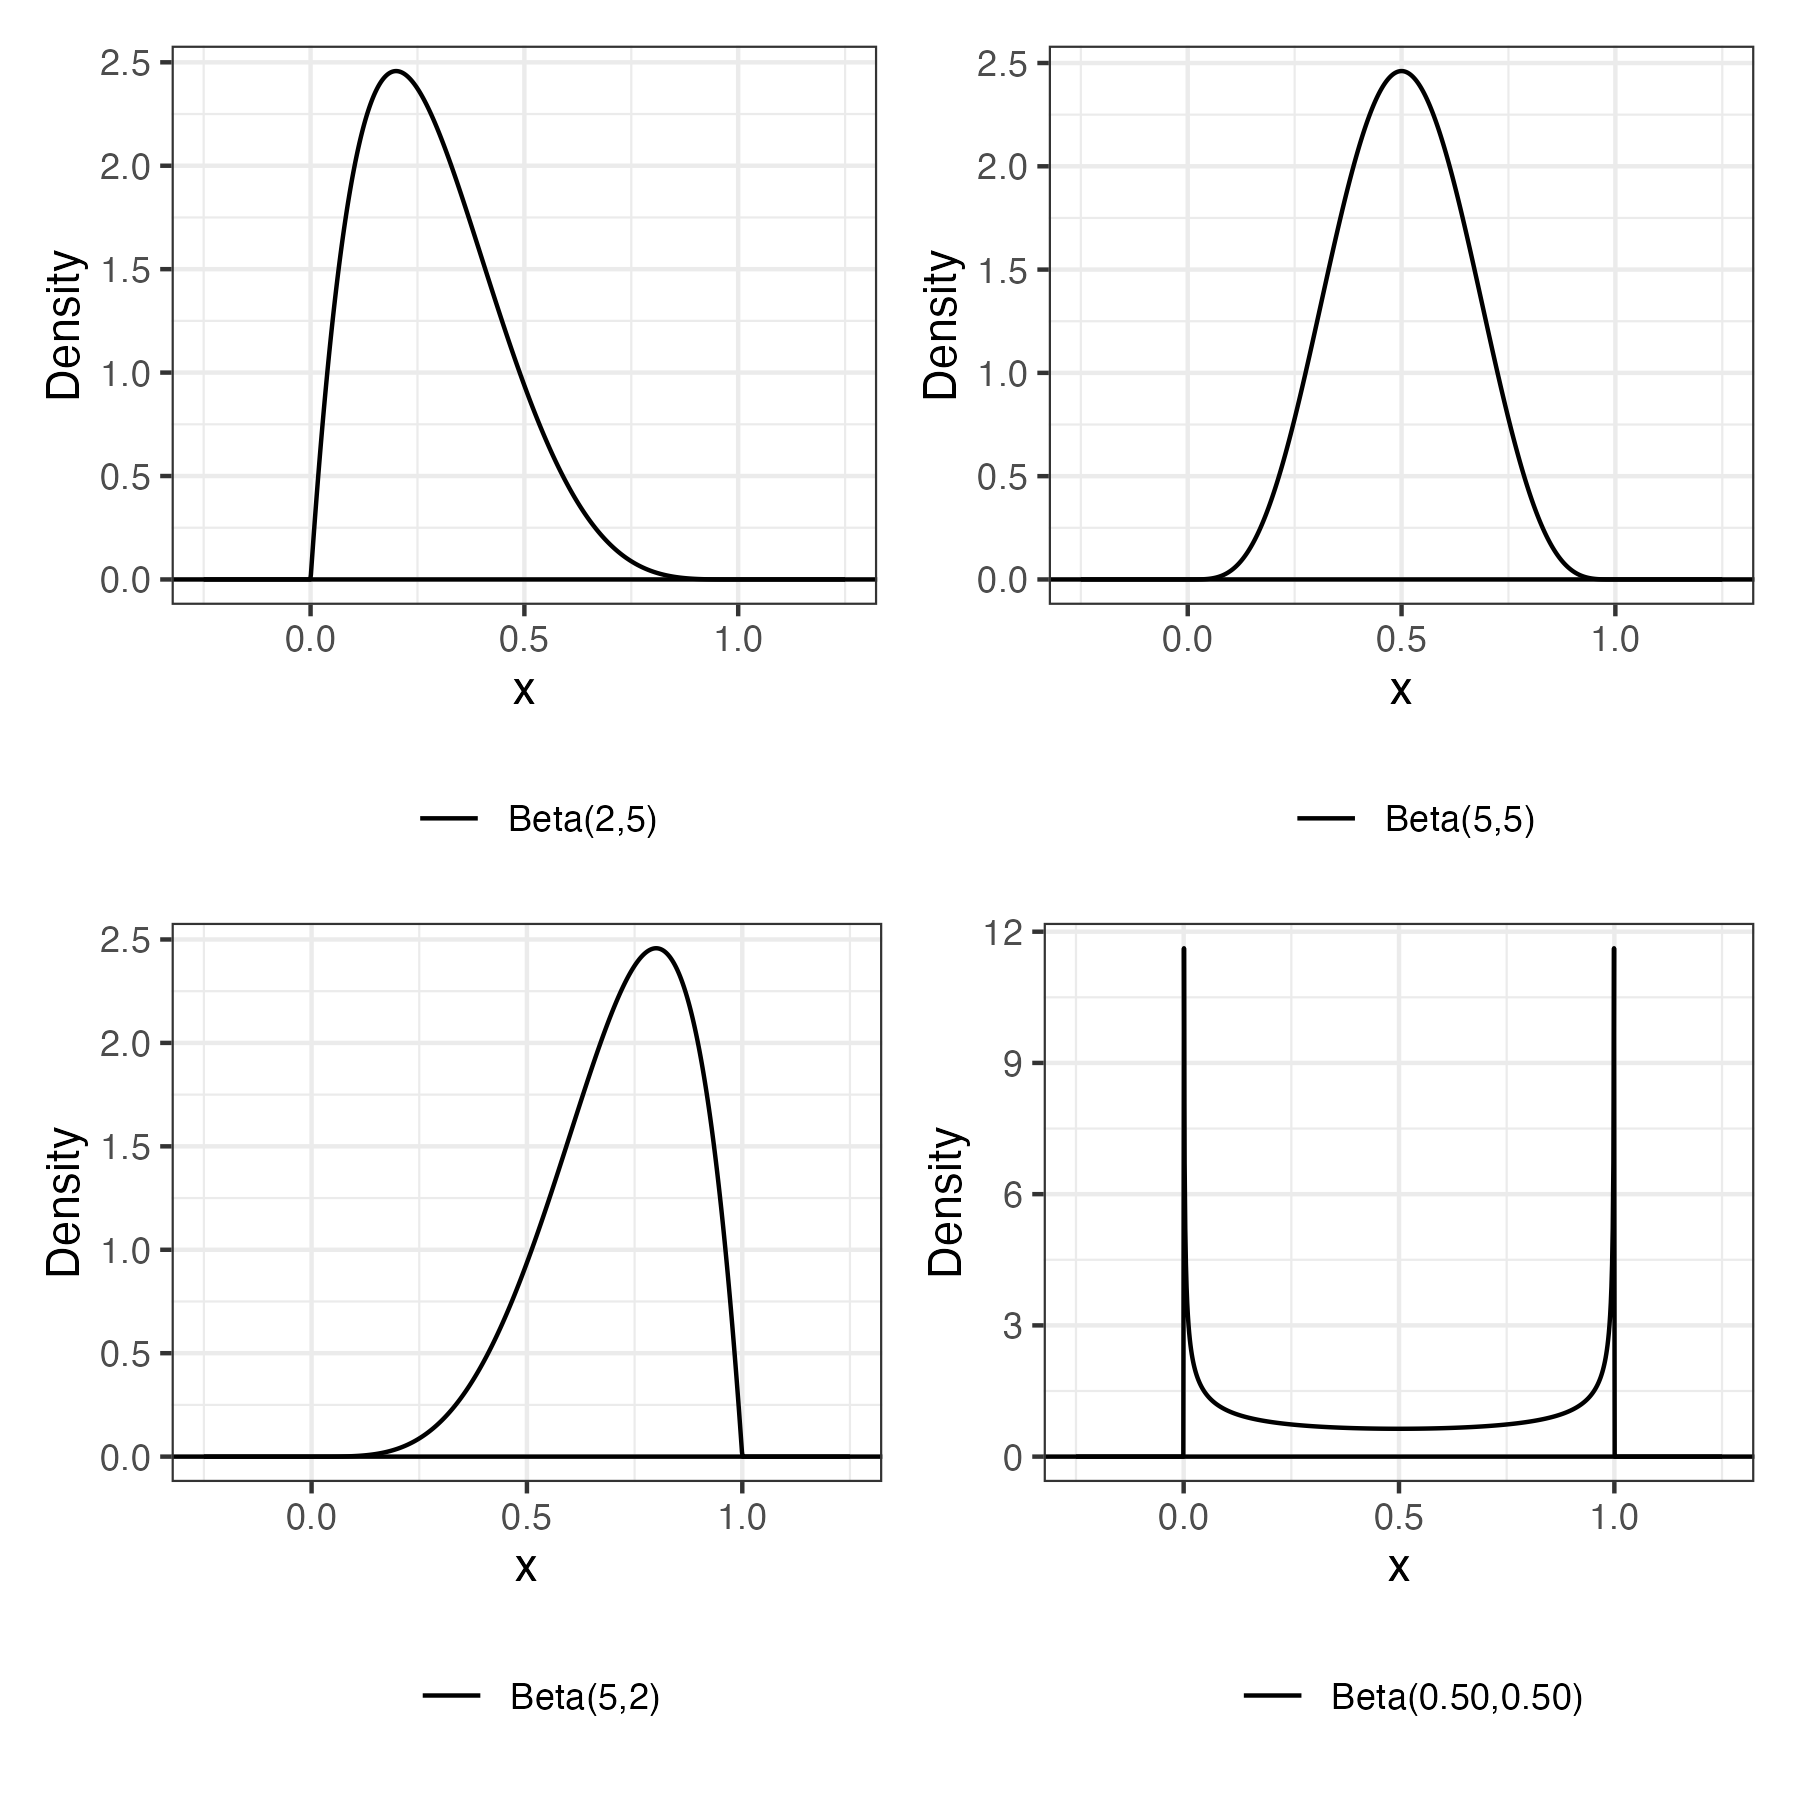
\includegraphics[width=\linewidth]{betaplots.png}
 \captionof{figure}{Beta distribution PDFs for different parameter values of $\alpha$ and $\beta$}
 \label{fig:betaplots}
\end{Figure}

The four plots in Figure (\ref{fig:betaplots}) illustrate Beta probability density function with various combinations of parameters $\alpha$ and $\beta$. The top-left plot demonstrates a distribution skewed to the right (where $\beta > \alpha$), so there is a higher chance of observing values in the lower range of the interval [0,1]. The top-right plot demonstrates a symmetric distribution centered around 0.5 ($\alpha = \beta$). Here, the values in the middle of the interval are most likely to occur. The bottom-left plot demonstrates a left-skewed distribution(where $\alpha > \beta$). The values closer to the end of the interval are most likely to occur. The bottom-right plot illustrates a U-shaped distribution (both $\alpha, \beta < 1$). The density is highest at the endpoints of the interval and lowest around 0.5.


\section{Properties}\label{sec:prop}

The Beta distribution has the following key properties:
\begin{itemize}
    \item Mean: 
    $$E(X) = \frac{\alpha}{\alpha + \beta}$$

    \item Variance:
    $$\text{var}(X) = \frac{\alpha \beta}{(\alpha + \beta)^2 (\alpha + \beta + 1)}$$

    \item Skewness:
    $$\text{skew}(X) = \frac{2(\beta - \alpha)\sqrt{\alpha + \beta + 1}}{(\alpha + \beta + 2)\sqrt{\alpha \beta}}$$

    \item Excess Kurtosis:
    $$\text{kurt}(X) = \frac{6[(\alpha - \beta)^2(\alpha + \beta + 1) - \alpha \beta(\alpha + \beta + 2)]}{\alpha \beta (\alpha + \beta + 2)(\alpha + \beta + 3)}$$
\end{itemize}

Based on Figure (\ref{fig:betaplots}), we can see the values of the mean, variance, skewness, and excess kurtosis in Table (\ref{statsProperties.tab}). The mean of the distribution reflects the average value of the distribution. A low mean (such as for Beta(2, 5)) indicates a right-skewed distribution and a high mean (such as for Beta(5, 2)) indicates a left-skewed distribution. The mean when parameters $\alpha = \beta$ indicates a symmetrical distribution (Beta(5,5)). 

The variance indicates the spread of the distribution around the mean. Beta(5,5) has the lowest variance and Beta(0.5,0.5) has the highest variance.

The skewness describes the asymmetry of the distribution. Positive skewness indicates a right-skewed distribution (Beta(2,5)) and negative skewness indicates a left-skewed distribution (Beta(5,5)). If skewness is zero, the distribution is symmetric (Beta(0.5,0.5) and Beta(5,5)).

The excess kurtosis measures how peaked the distribution is compared to a normal distribution. If it is equal to 0, the distribution is as peaked as the normal distribution is (mesokurtic). If it is positive, the distribution has a sharp peak and flat tails (leptokurtic). If excess kurtosis is negative, the distribution has a plat peak and thin tails (platykurtic). All four Beta distributions analyzed are platykurtic.

\section{Estimators}\label{sec:estim}

Given a sample drawn from Beta distribution, we can estimate parameters $\alpha$ and $\beta$ using the method of moments (MOM) and maximum likelihood estimation (MLE).

To estimate $\alpha$ and $\beta$ using MOM, we need to equate the first two sample moments ($E(X), E(X^2)$) to the population moments.

The mean (first moment) of the Beta distribution is:
$$E(X) = \frac{\alpha}{\alpha + \beta}$$

The variance (related to the second moment) of the Beta distribution is:
$$E(X^2) = \frac{\alpha \beta}{(\alpha + \beta)^2 (\alpha + \beta + 1)}$$

To estimate $\alpha$ and $\beta$ using by computing maximum likelihood estimation, we need to maximize the likelihood function based on the observed data. To simplify the optimization process, we can maximize the log-likelihood.

The log-likelihood function:
$$L(\alpha, \beta | X) = \prod_{i=1}^{n} f_X(x_i| \alpha, \beta)$$

In Section \ref{sec:examp} we examine death rates data using Beta distribution. The estimates for shape parameters $\alpha$ and $\beta$ based on the death data from the World Bank were computed using both MOM and MLE and we can see estimates' densities in Figure (\ref{fig:mommle}).

\begin{Figure}
 \centering
 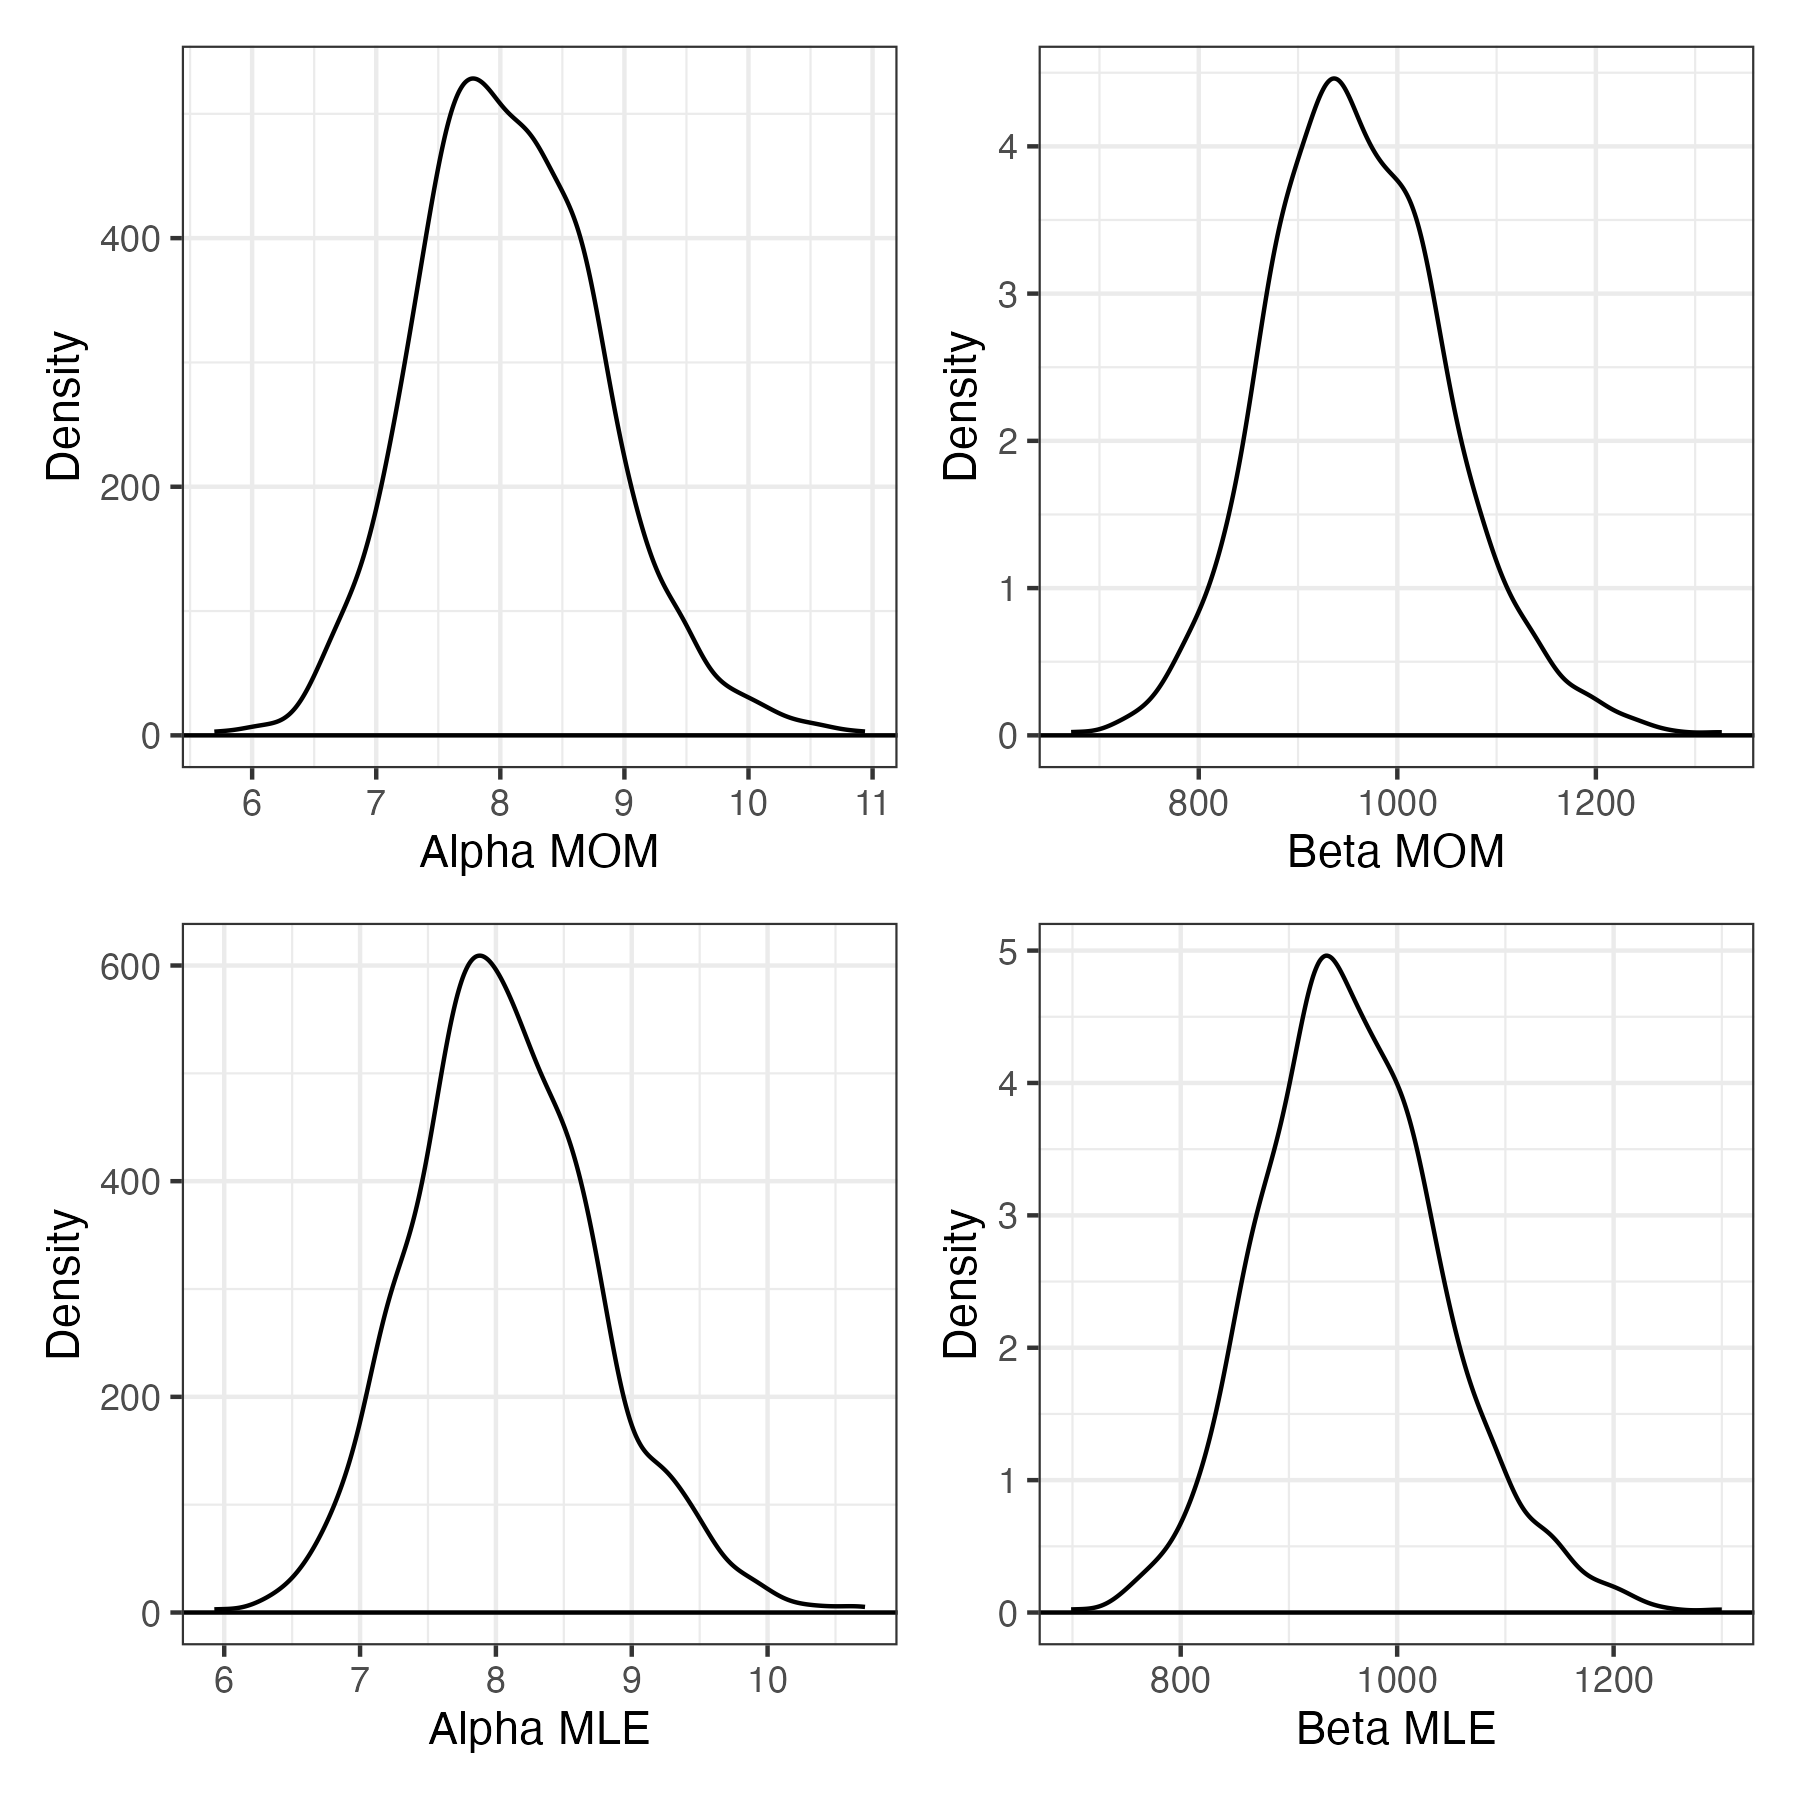
\includegraphics[width=\linewidth]{mommle.png}
 \captionof{figure}{Density of estimates for $\alpha$ and $\beta$ using MOM and MLE}
 \label{fig:mommle}
\end{Figure}

We can see that the distributions of the estimated parameters are similar in shape. However, there is a slight difference in peak locations for MOM and MLE estimates. MLE has slightly lower means and significantly lower variability compared to MOM estimates.

We also computed bias, precision, and mean squared error for estimates in Figure (\ref{fig:mommle}). The numerical estimates are provided in Table (\ref{precision.tab}). It is evident that MLE provides lower bias, higher precision, and lower mean squared error for both $\alpha$ and $\beta$ estimates.

In our example, MLE has a smaller variance, higher precision, and lower bias compared to MOM, so MLE should be the preferred estimator.


\section{Example}\label{sec:examp}
As an example of application for the Beta distribution, consider country death rates. We draw the data set from the World Bank and convert the data to a rate of number of deaths per 1000 citizens to satisfy the interval $X \in [0,1]$.

\begin{Figure}
 \centering
 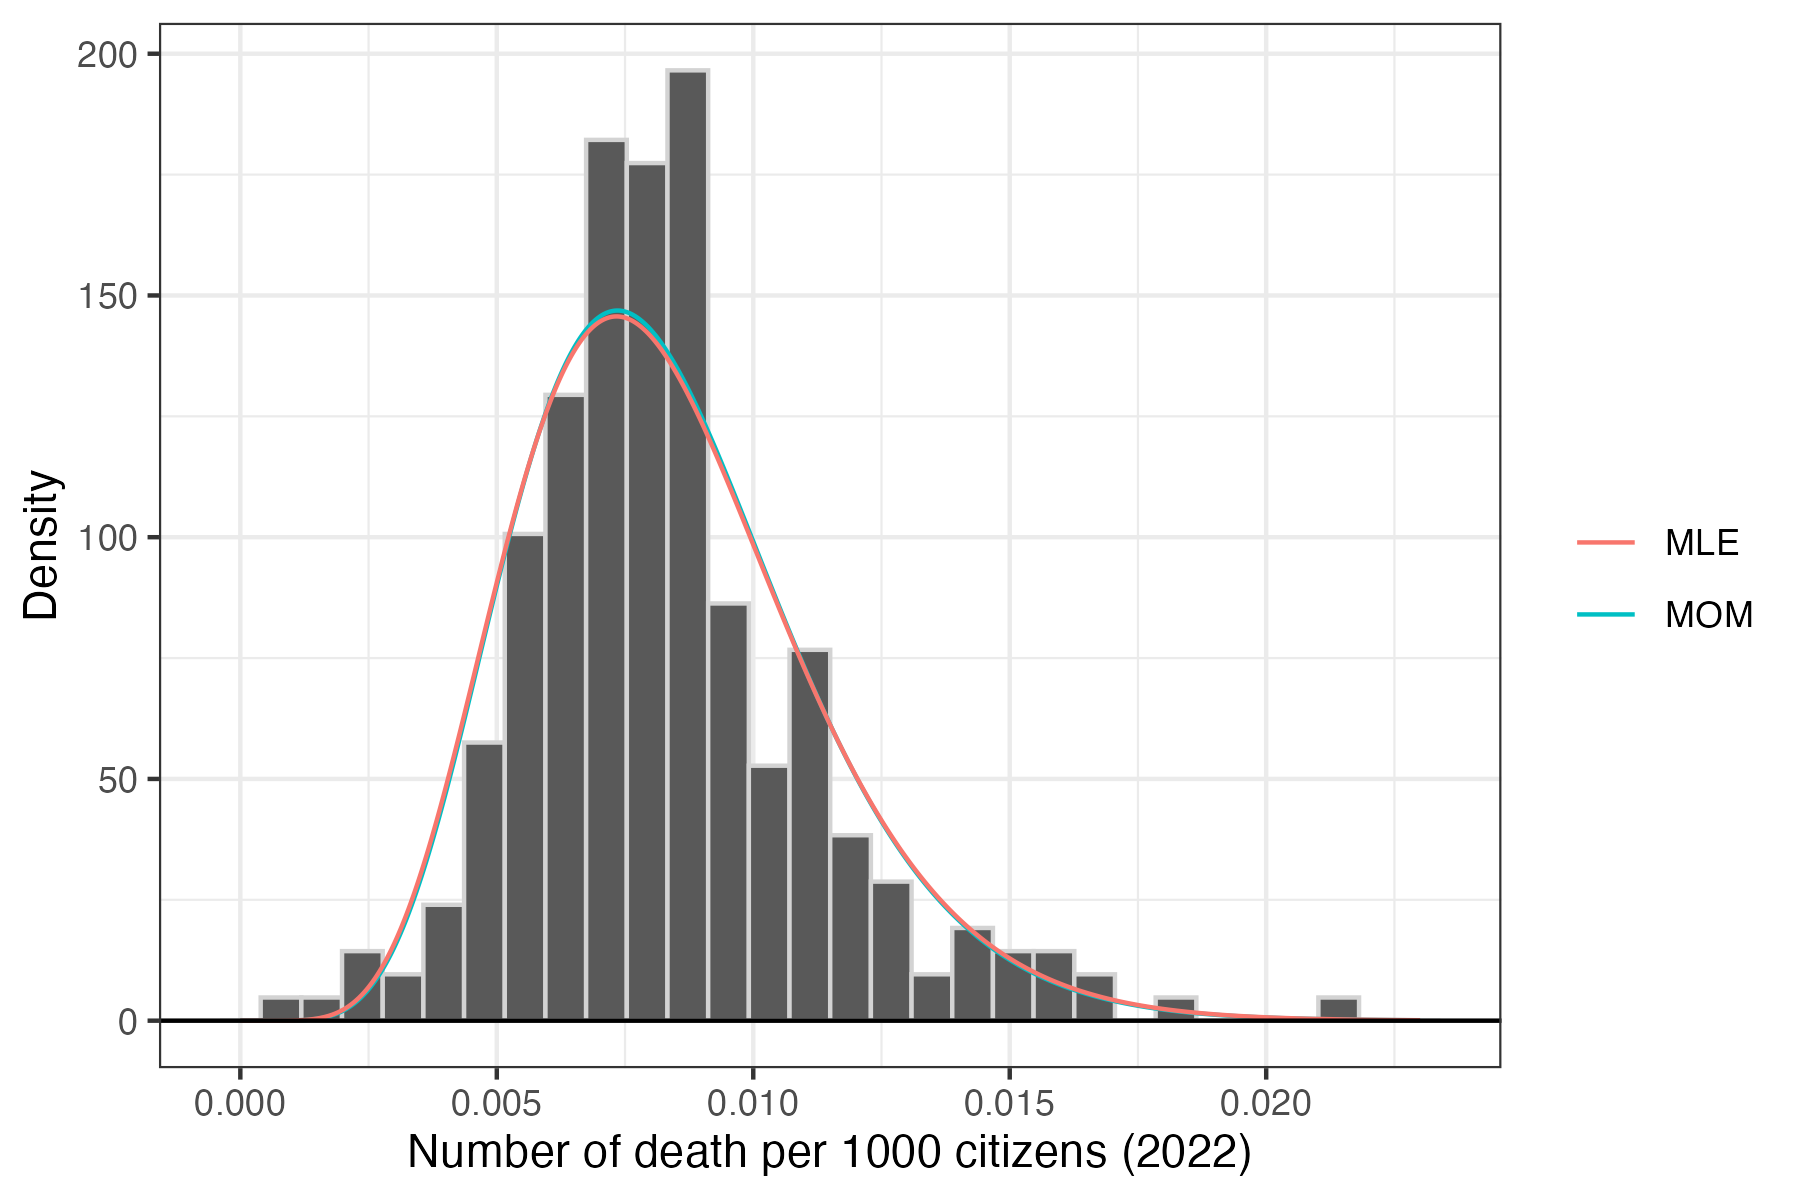
\includegraphics[width=\linewidth]{deathdata.png}
 \captionof{figure}{Histogram of death rates with MOM and MLE distributions superimposed}
 \label{fig:deathdata}
\end{Figure}


\subsection{Methods Subsection}
Describe the data you are working with, if applicable. Describe the specific process you will follow to answer the question at hand. This does not mean you should write something like this.
\begin{quote}
\textit{I did this and then I did that and then I did this other thing and then..., and then..., and then...}
\end{quote}
Instead, it should provide a clear and concise narrative that flows from the problem specification in the Introduction to how you will approach answering it. This is where I would expect to see some citations for \texttt{R} packages you will use to conduct the statistical analysis reported in the Results section.
Much like the Introduction, subsections can be helpful for the Methods section. For example, you might describe data collection and the statistical analyses of the collected data in different subsections. Or, you may have different questions that require distinct methods. 

\section{Results}
Tie together the Introduction -- where you introduce the problem at hand -- and the methods --  what you propose to do to answer the question. Present your data, the results of your analyses, and how each reported aspect contributes to answering the question. This section should include table(s), statistic(s), and graphical displays. Make sure to put the results in a sensible order and that each result contributes a logical and developed solution. It should not just be a list. Avoid being repetitive. 

\subsection{Results Subsection}
Subsections can be helpful for the Results section, too. This can be particularly helpful if you have different questions to answer. 


\section{Discussion}
 You should objectively evaluate the evidence you found in the data. Do not embellish or wish-terpet (my made-up phase for making an interpretation you, or the researcher, wants to be true without the data \emph{actually} supporting it). Connect your findings to the existing information you provided in the Introduction.

Finally, provide some concluding remarks that tie together the entire paper. Think of the last part of the results as abstract-like. Tell the reader what they just consumed -- what's the takeaway message?

%%%%%%%%%%%%%%%%%%%%%%%%%%%%%%%%%%%%%%%%%%%%%%%%%%%%%%%%%%%%%%%%%%%%%%%%%%%%%%%%
% Bibliography
%%%%%%%%%%%%%%%%%%%%%%%%%%%%%%%%%%%%%%%%%%%%%%%%%%%%%%%%%%%%%%%%%%%%%%%%%%%%%%%%
\vspace{2em}

\noindent\textbf{Bibliography:} Note that when you add citations to your bib.bib file \emph{and}
you cite them in your document, the bibliography section will automatically populate here.

\begin{tiny}
\bibliography{bib}
\end{tiny}
\end{multicols}

%%%%%%%%%%%%%%%%%%%%%%%%%%%%%%%%%%%%%%%%%%%%%%%%%%%%%%%%%%%%%%%%%%%%%%%%%%%%%%%%
% Appendix
%%%%%%%%%%%%%%%%%%%%%%%%%%%%%%%%%%%%%%%%%%%%%%%%%%%%%%%%%%%%%%%%%%%%%%%%%%%%%%%%
\newpage
\onecolumn
\section{Appendix}

%creating an xtable for the properties
% latex table generated in R 4.4.2 by xtable 1.8-4 package
% Mon Mar 31 22:58:05 2025
\begin{table}[ht]
\centering
\begin{tabular}{|c|c|c|c|c|}
  \hline
Distribution & Mean & Variance & Skewness & Excess.Kurtosis \\ 
  \hline
Beta(2,5) & 0.29 & 0.03 & 0.60 & -0.12 \\ 
  Beta(5,5) & 0.50 & 0.02 & 0.00 & -0.46 \\ 
  Beta(5,2) & 0.71 & 0.03 & -0.60 & -0.12 \\ 
  Beta(0.5,0.5) & 0.50 & 0.12 & 0.00 & -1.50 \\ 
   \hline
\end{tabular}
\caption{Statistical properties for various parameteres of Beta distribution} 
\label{statsProperties.tab}
\end{table}


% latex table generated in R 4.4.2 by xtable 1.8-4 package
% Mon Mar 31 22:58:05 2025
\begin{table}[ht]
\centering
\begin{tabular}{|c|c|c|c|}
  \hline
Estimate & Bias & Precision & Mean.Squared.Error \\ 
  \hline
Alpha MOM & 0.08 & 1.83 & 0.55 \\ 
  Beta MOM & 10.57 & 0.00 & 8303.00 \\ 
  Alpha MLE & 0.07 & 2.13 & 0.47 \\ 
  Beta MLE & 9.18 & 0.00 & 7118.73 \\ 
   \hline
\end{tabular}
\caption{Bias, precision, and mean squared error for estimates} 
\label{precision.tab}
\end{table}


\end{document}
